\subsubsection*{Conventional versus modern neuroscience experimentation}

Conventional system neuroscience experiments heavily constrain the behaviour of
their subjects in order to simplify behavioural and neural analysis.  However,
important aspects of brain function may not be expressed in these constrained
behaviours and these aspects may only manifest in naturalistic experimental
conditions.

% recent foraging experiments
% -> need of advanced machine learning methods to extract information from these experiments

Recent technological advances now allow to build complex naturalistic
experiments, while measuring a large number of experimental variables and
recording from a large number of neurons simultaneously. These advances
allow unrestrained subjects behaviour with precise monitoring of what happens in
the subjects' environment and brain.

Important examples of these experiments are naturalistic foraging experiments,
where freely moving subjects search for food in unrestrained environments.
Foraging studies are currently underway at major research centres around the
world (e.g., the Allen Institute for Brain Research, Janelia Farm, the Max
Plank Institute of Animal Behaviour).

A complication of naturalistic neuroscience experiments is extracting meaning
from the plethora of data that they generate \citep{juavinett22}. Machine
learning methods are specially helpful to address this problem. For example,
they can be used to extract subjects' internal states from behavioural
measurements, to extract low-dimensional latent variables from high-dimensional
neural recordings, and to relate the inferred subjects' internal state to the
neural latent variables.

The data generated by conventional system neuroscience experiments can be
understood by just plotting a few of its variables. However, interpreting the output
of naturalistic experiments is more difficult and machine learning methods
become essential for this.

\subsubsection*{Long-duration and naturalistic experiments at the SWC}
% at the SWC we are performing a new type of foraging experminets

At the SWC we are performing a novel type of naturalistic and long-duration
foraging experiments. Mice are housed in large circular arenas
(Figure~\ref{fig:arena}a)
equipped with a shelter, where animals can rest and drink, and with food patches,
where animals can get food pellets after moving a wheel for a fixed
configurable distance (Figure~\ref{fig:arena}b). Mice live in the arena for extended periods of time. We
monitor the behaviour of mice in detail with multiple high-resolution video
cameras, to monitor the positions of mice body parts, ultrasound audio cameras,
to monitor mice vocalisations, and a scale in the shelter, to regularly measure
mice weights. We record neural activity using Neuropixel probes with 5,000
channels, from which 384 channels can be selected for recording, and with
64-channel probes, equipped with an electrical stimulator and an optical
stimulator.
%
We running foraging experiments with one or multiple mice per arena.

\begin{figure}
    \centering
    \begin{subfigure}{\textwidth}
        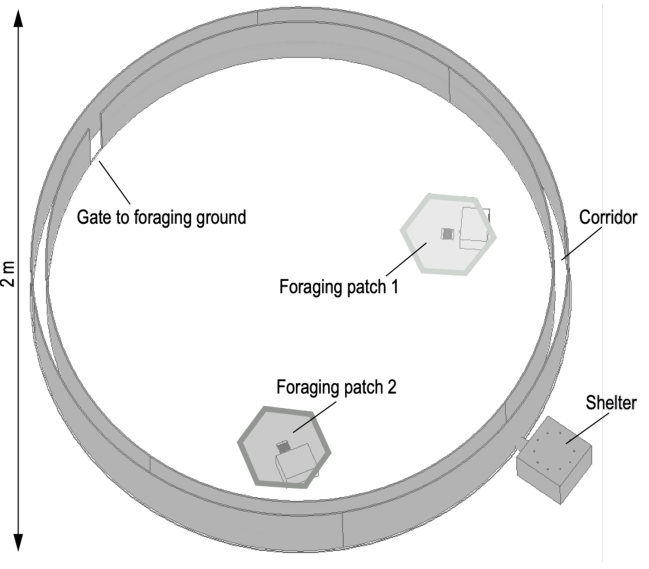
\includegraphics[width=4in]{figures/arena.png}
        \caption{}
    \end{subfigure}
    \begin{subfigure}{\textwidth}
        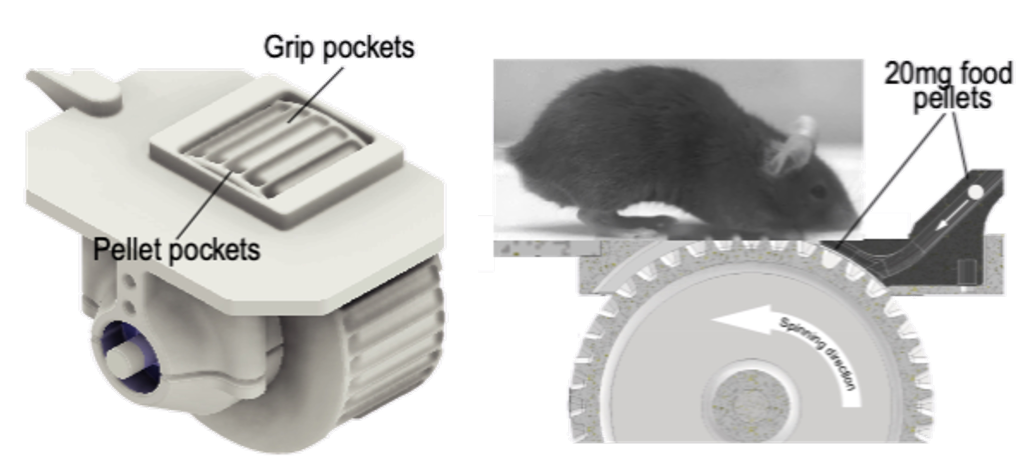
\includegraphics[width=4in]{figures/patch.png}
        \caption{}
    \end{subfigure}
    \caption{Foraging arena (a) and patch (b).}
    \label{fig:arena}
\end{figure}

A unique feature of our foraging experiments is their long duration. We have
already recorded behaviour and neural activity of mice continuously for 48 hours
and by the end of 2024 we aim at recording continuously for two weeks.

These long-duration experiments are allowing us to address foraging questions
that cannot be studied in shorter experiments. For example, scientifically
these experiments allow us to ask how do mice foraging patterns change across
days, and what are the neural mechanisms underlying these changes.
Statistically, the large amount of data recorded in the new experiments allows
us to estimate parameters of much more complex models than those that can be
fitted to data from conventional system neuroscience experiments.

% normative versus statistical characterization of foraging behavior
% The most common characterization of foraging experiments is a principled one,
% based on the marginal value theorem~\citep{charnov74}. It states that a subject
% will leave a patch when the reward rate of the patch falls below the average
% reward rate in the environment. Naturalistic and long-duration experiments
% allow us to attemp statistical characterizations of foraging experiments

% The naturalistic and long-duration experiments

\subsubsection*{Proposed resource}
% the proposed project

Here we propose to create a resource to (1) share data from our long-duration
naturalistic foraging experiments, (2) share machine learning software
implementations of methods to simulate and analyze these data and (3) organize
foraging data simulations and analysis competitions (Figure~\ref{fig:resource}).

\begin{figure}
    \begin{center}
        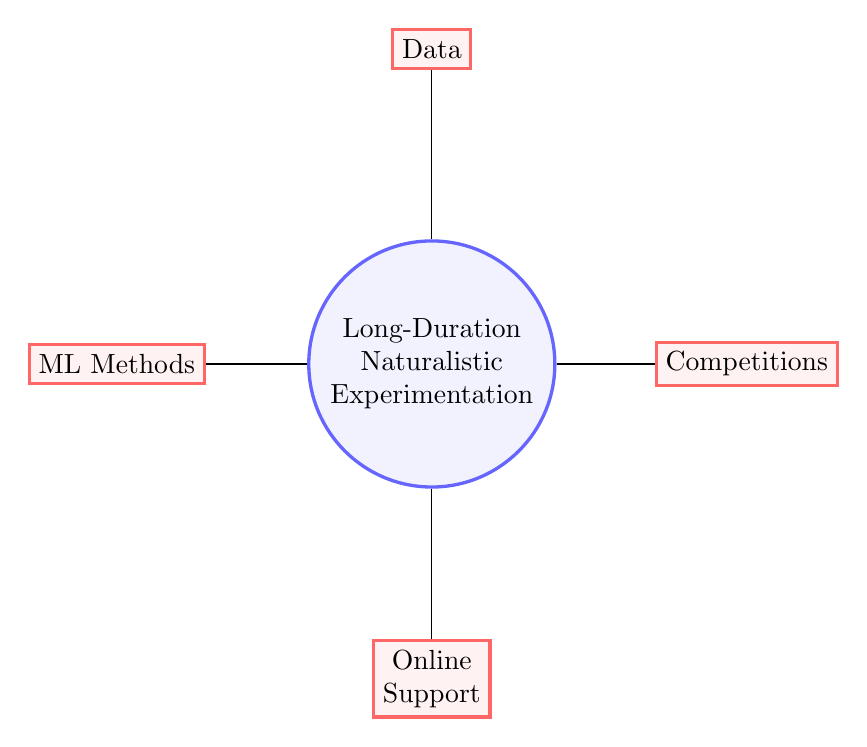
\begin{tikzpicture}[
        node distance=4cm and 1cm,
        centralNode/.style={circle, draw=blue!60, fill=blue!5, very thick,
        minimum size=7mm, align=center},
        itemNode/.style={rectangle, draw=red!60, fill=red!5, very thick,
        minimum size=5mm, align=center},
    ]
    \node[centralNode] (ldnExp)                                 {Long-Duration\\Naturalistic\\Experimentation};
    \node[itemNode]    (dataRepo)           [above of=ldnExp]   {Data};
    \node[itemNode]    (methodsRepo)        [left of=ldnExp]    {ML Methods};
    \node[itemNode]    (competitionsRepo)   [right of=ldnExp]   {Competitions};
    \node[itemNode]    (onlineSupport)      [below of=ldnExp]   {Online\\Support};
    \draw[-] (ldnExp) -- (dataRepo);
    \draw[-] (ldnExp) -- (methodsRepo);
    \draw[-] (ldnExp) -- (competitionsRepo);
    \draw[-] (ldnExp) -- (onlineSupport);
\end{tikzpicture}

    \end{center}
    \caption{Resource theme (blue) and deliverables (red).}
    \label{fig:resource}
\end{figure}

Data generated by our long-duration and naturalistic foraging experiments will
be made publicly available, following FAIR standards, in the
\href{https://dandiarchive.org/}{DANDI} archive.

Whenever possible we will distribute offline and online implementations of all
data analysis methods. These methods will be thoroughly evaluated with shared
data.
%
We will initially distribute methods that we have used for our foraging
experiments. For several functionalities we have used more than one method, and
we will distribute all of them. In this way experimental neuroscientists using
our resource should be able to compare different distributed methods and choose
the one more suitable to their needs.

We will welcome contributions from machine learning method developers
interested in applying their methods to data generated by our foraging
experiments. To encourage them we will organize data
competitions where participants will be given a data problem to solve (e.g., to
simulate a given environment or to analyze a given dataset), they will provide
their solutions, and we will select the winning one.

\subsubsection*{Intelligent experimental control with Bonsai}

Bonsai is a reactive visual programming environment developed by NeuroGEARS Ltd
that is widely used in Neuroscience for controlling sophisticated neuroscience
experiments. Reactive programs are very different from procedural ones (like C
or Python). The main entity of a reactive program is stream and a reactive
program is a sequence of stream transformations that get an input stream,
transform it, and generate an output one. Reactive programs are ideal to
process online data, like those generated in animal neuroscience experiments.

Funded by a BBR
award\footnote{\url{https://gow.bbsrc.ukri.org/grants/AwardDetails.aspx?FundingReference=BB\%2FW019132\%2F1}}
we at the SWC, GCNU and NeuroGEARS are adding machine learning methods to
Bonsai. A central goal is to allow Bonsai to control neuroscience experiments
based on inferences performed online on behavioral and neural data.

Not all algorithms that we propose to distribute in this resource admit and
online implementation, however most of them do. Whenever possible, we will
distribute online versions of the distributed methods implemented in Bonsai.

\subsubsection*{Resource background}

In July 2020 the SWC began building hardware and software infrastructure to
record behaviour and neural actvity of freely moving mice foraging in large
arenas. Our initial focus was on monitoring behavior for extended periods of
time. We have been able to monitor mice positions, their food consumption and
weight for up to xx weeks in experiment with different food delivery policies.

More recently we have been able to record behavior (as described above) and
neural activty (Neuropixel array, four shanks, 384 electrodes per shank) for up
to 48 hours.

We have developed computer vision methods to track the center of mass of
foraging mice, linear dynamical methods to infer mice kinematics (e.g.,
velocity and acceleration) from tracked positions and Hidden Markov Models to
infer mice states from kinematics inferences.
%
We have also linear and nonlinear regression models to predict mice patch
visit durations from inferred kinematics and states.

We have not yet processed neural recordings from the foraging experiment.
However, at the GCNU we have extensive experience developing and applying
advanced statistical models for neural recordings, which will expedite our
processing of neural foraging data.

We expect that a position paper describing our foraging experiments will be
published by ??/????

\subsubsection*{Why is the proposed resource unique and timely}

% why is the resource unique and timely

Long-duration and naturalistic experimentation is the future of experimental
neuroscience.  Animal foraging is a central neuroscience problem today and
multiple groups around the world are working on it (e.g., Allen Institute for
Neural Dynamics, Janelia Farm, University of Konstanz). Yet, none of this
groups is focused on the unique long-duration and naturalistic experiments that
we are developing at the SWC. It is imperative for the UK to become a leader on
this new type of experimentation. The foraging data and the machine learning
methods that we propose to distribute are key elements for world-class foraging
research.

The US Brain Research through Advancing Innovative Neurotechnologies (BRAIN)
initiative~\citep{jorgensonEtAl15} funded projects focused on data analysis
with advanced machine learning methods for long-duration and complex experiment
that we propose to address in this project. However, none BRAIN initiative
project generated the unique long-duration and naturalistic neuroscience
experimental data that we are creating at the SWC.

We (the SWC, GCNU and NeuroGEARS) are an excellent team to develop the proposed
resource. The SWC is at the forefront of experimental neuroscience research and
has been developing mice foraging experiments for five years. The GCNU is a
leader in computational neuroscience and machine learning, with ample
experience in building methods to characterize neural data, and more recently
in distributing openly machine learning methods. And NeuroGEARS has more than a
decade of experience building high-quality software for experimental
neuroscience. We collaborate extensively in a wide range of projects.

